\documentclass[12pt, a4paper]{article}
\usepackage{../notesheets}
%%%%%%%%%%%%%%%%%%%%%%%%%%%%%%%%%%%%%%%%%%%%%%%%%% 
\author{Math 1220}
\title{Notesheet. Section 8.3: Maxima and Minima of Function of
  Several Variables}
\date{}

\begin{document}
\maketitle
\nameline
%%%%%%%%%%%%%%%%%%%%%%%%%%%%%%%%%%%%%%%%%%%%%%%%%%
\vspace{0.5in}
\begin{defi}
  Let \(f(x,y)\) be a function defined on a region \(R\) containing
  the point \((a,b)\). Then,
  \begin{itemize}
  \item \(f\) has a \de{relative maximum at \((a,b)\)} with
    \de{relative maximum value} \(f(a,b)\) if \\
    
  \item \(f\) has a \de{relative minimum at \((a,b)\)} with
    \de{relative minumum value} \(f(a,b)\) if\\
    
  \item \(f\) has an \de{absolute maximum at \((a,b)\)} with
    \de{absolute maximum value} \(f(a,b)\) if\\
    
  \item \(f\) has an \de{absolute minimum at \((a,b)\)} with
    \de{absolute minimum value} \(f(a,b)\) if
  \end{itemize}
\end{defi}
\begin{ex}
  Consider the function \(f(x,y) = x^2 + y^2\). Does this function
  have any relative minima? Relative maxima? What is
  \(f_x(0,0)\) and \(f_y(0,0)\)?
\end{ex}
\begin{thrm}
  If \(f(x,y)\) is a differentiable function of two variables and has
  a relative maximum (relative minimum) at a point \((a,b)\) in the
  domain of \(f\), then 
\end{thrm}
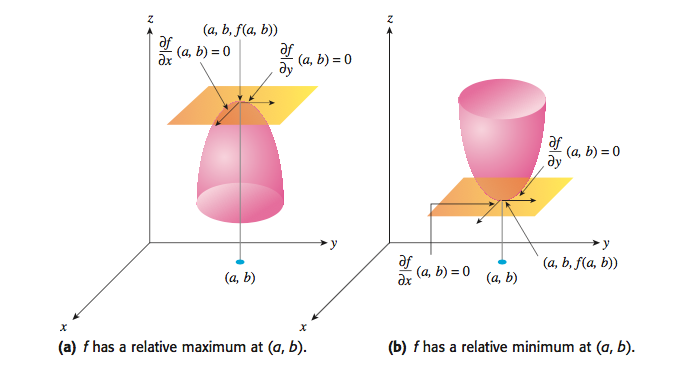
\includegraphics[scale=0.5]{images/local-min-max}
\begin{defi}
  A \de{critical point} is a point where 
\end{defi}
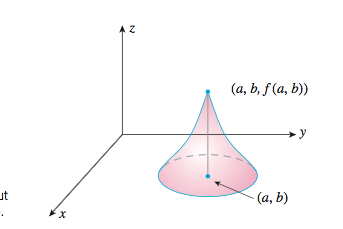
\includegraphics[scale=0.5]{images/critical-pt-deriv-dne} 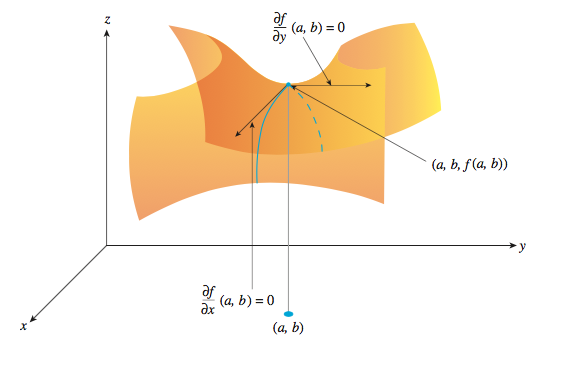
\includegraphics[scale=0.35]{images/saddle-point}
\begin{defi}
  A \de{saddle point} is a point where 
\end{defi}
%%%%%%%%%%%%%%%%%%%%%%%%%%%%%%%%%%%%%%%%%%%%%%%%%% 
\end{document}
